% PRL look and style (easy on the eyes)
\documentclass[aps,pre,twocolumn,nofootinbib,superscriptaddress,linenumbers]{revtex4-1}
% Two-column style (for submission/review/editing)
%\documentclass[aps,prl,preprint,nofootinbib,superscriptaddress,linenumbers]{revtex4-1}

%\usepackage{palatino}

%\usepackage{palatino}
% Change to a sans serif font.
\usepackage{sourcesanspro}
\renewcommand*\familydefault{\sfdefault} %% Only if the base font of the document is to be sans serif
\usepackage[T1]{fontenc}
%\usepackage[font=sf,justification=justified]{caption}
\usepackage[font=sf]{floatrow}

% Rework captions to use sans serif font.
\makeatletter
\renewcommand\@make@capt@title[2]{%
 \@ifx@empty\float@link{\@firstofone}{\expandafter\href\expandafter{\float@link}}%
  {\sf\textbf{#1}}\sf\@caption@fignum@sep#2\quad
}%
\makeatother

\usepackage{listings} % For code examples
\usepackage[usenames,dvipsnames,svgnames,table]{xcolor}

\usepackage{amsmath}
\usepackage{amssymb}
\pdfoutput=1
\usepackage[pdftex]{graphicx}
%\usepackage[mathbf,mathcal]{euler}
%\usepackage{citesort}
\usepackage{dcolumn}
\usepackage{boxedminipage}
\usepackage{verbatim}
\usepackage[colorlinks=true,citecolor=blue,linkcolor=blue]{hyperref}
\usepackage[group-separator={,}]{siunitx}


% The figures are in a figures/ subdirectory.
% \graphicspath{{figures/}}


% \newcommand{\pyitc}{\url{http://www.simtk.org/home/bayesian-itc}} % URL of pyITC project homepage

%% DOCUMENT %%%%%%%%%%%%%%%%%%%%%%%%%%%%%%%%%%%%%%%%%%%%%%%%%%%%%%%%%%%%%%%%%%%%
\begin{document}

%% TITLE %%%%%%%%%%%%%%%%%%%%%%%%%%%%%%%%%%%%%%%%%%%%%%%%%%%%%%%%%%%%%%%%%%%%
\title{Ensembler: Enabling high-throughput molecular simulations at the superfamily scale}

\author{Daniel L. Parton}
  \affiliation{Computational Biology Program, Sloan Kettering Institute, Memorial Sloan Kettering Cancer Center, New York, NY 10065}
  %\email{daniel.parton@choderalab.org}
\author{Patrick B. Grinaway}
  \affiliation{Computational Biology Program, Sloan Kettering Institute, Memorial Sloan Kettering Cancer Center, New York, NY 10065}
  %\email{patrick.grinaway@choderalab.org}
\author{John D. Chodera}
 \thanks{Corresponding author}
 \email{john.chodera@choderalab.org}
  \affiliation{Computational Biology Program, Sloan Kettering Institute, Memorial Sloan Kettering Cancer Center, New York, NY 10065}

\date{\today}

%%%%%%%%%%%%%%%%%%%%%%%%%%%%%%%%%%%%%%%%%%%%%%%%%%%%%%%%%%%%%%%%%%%%%%%%%%%%%%%%%%%%%%%%%%%%%%%%%%%%%%
% ABSTRACT/pacs
%%%%%%%%%%%%%%%%%%%%%%%%%%%%%%%%%%%%%%%%%%%%%%%%%%%%%%%%%%%%%%%%%%%%%%%%%%%%%%%%%%%%%%%%%%%%%%%%%%%%%%
\begin{abstract}

The rapidly expanding body of available genomic and protein structural data provides a rich resource for understanding protein dynamics with biomolecular simulation. 
While computational infrastructure has grown rapidly, simulations on an \emph{omics} scale are not yet widespread, primarily because software infrastructure to enable this has not kept pace. 
It should now be possible to study protein dynamics across entire (super)families, exploiting the variety of available structural biology data and conformational similarities across homologous proteins.
Here, we present a new tool for enabling high-throughput simulation in the genomics era.
{\bf Ensembler} takes any set of sequences---from a single sequence to an entire superfamily---and shepherds them through various stages of modeling and refinement to produce simulation-ready structures.
This includes comparative modeling to all relevant PDB structures (which may span multiple conformational states of interest), reconstruction of missing loops, addition of missing atoms, culling of nearly identical structures, assignment of appropriate protonation states, solvation in explicit solvent, and refinement with molecular simulation to ensure stable simulation. 
The output of this pipeline is an ensemble of structures ready for subsequent molecular simulations using computer clusters, supercomputers, or distributed computing projects like Folding@home.
{\bf Ensembler} automates much of the time-consuming process of preparing protein models suitable for simulation, while allowing scalability up to entire superfamilies.  
A particular advantage of this approach can be found in the construction of kinetic models of conformational dynamics---such as Markov state models---which benefit from a diverse array of initial configurations that span the accessible conformational states to aid sampling.
We demonstrate the power of this approach by constructing models for all catalytic domains in the human tyrosine kinase family, using all available kinase catalytic domain structures from any organism as structural templates.

{\bf Ensembler} is free and open source software licensed under the GNU General Public License (GPL) v2. 
It should run on all major operating systems, and has been tested on Linux and OS X.
The latest release can be installed via the {\tt conda} package manager, and the latest source can be downloaded from \url{https://github.com/choderalab/ensembler}.

\emph{Keywords: molecular dynamics simulation; comparative modeling}

% TODO expand to all human protein kinases?

\end{abstract}

\maketitle

%%%%%%%%%%%%%%%%%%%%%%%%%%%%%%%%%%%%%%%%%%%%%%%%%%%%%%%%%%%%%%%%%%%%%%%%%%%%%%%%%%%%%%%%%%%%%%%%%%%%%%
% INTRODUCTION
%%%%%%%%%%%%%%%%%%%%%%%%%%%%%%%%%%%%%%%%%%%%%%%%%%%%%%%%%%%%%%%%%%%%%%%%%%%%%%%%%%%%%%%%%%%%%%%%%%%%%%
\section{Introduction}
\label{section:introduction}

Recent advances in genomics and structural biology have helped generate an enormous wealth of protein data at the level of amino-acid sequence and three-dimensional structure.
However, proteins typically exist as an ensemble of thermally accessible conformational states, and static structures provide only a snapshot of their rich dynamical behavior.
Many functional properties---such as the ability to bind small molecules or interact with signaling partners---require transitions between states, encompassing anything from reorganization of sidechains at binding interfaces to domain motions to large scale folding-unfolding events.
Drug discovery could also benefit from a more extensive consideration of protein dynamics, whereby small molecules might be selected based on their predicted ability to bind and trap a protein target in an inactive state [CITE Lee Craik Science 2009].

Molecular dynamics (MD) simulations have the capability, in principle, to describe the time evolution of a protein in atomistic detail, and have proven themselves to be a useful tool in the study of protein dynamics.
A number of mature software packages and forcefields are available, and much recent progress has been driven by advances in computing architecture.
For example, many MD packages are now able to exploit GPUs, which provide greatly improved simulation efficiency per unit cost relative to CPUs, while distributed computing platforms such as Folding@home [CITE], GPUGrid [CITE], and Copernicus [CITE] allow scalability on an unprecedented level.
In parallel, methods for building human-understandable models of protein dynamics from noisy simulation data, such as Markov state modeling (MSM) approaches, are now reaching maturity [CITE MSM reviews].
MSM methods in particular have the advantage of being able to aggregate data from multiple independent MD trajectories, facilitating parallelization of production simulations and thus greatly alleviating overall computational cost.
There also exist a number of mature software packages for comparative modeling of protein structures, in which a target protein sequence is modeled using one or more structures as templates [CITE Modeller and Rosetta and a recent homology modeling review].

However, it remains difficult for researchers to exploit the full variety of available protein sequence and structural data in simulation studies, largely due to limitations in software architecture.
For example, the set up of a biomolecular simulation is typically performed manually, encompassing a series of fairly standard (yet time-consuming) steps such as the choice of protein sequence construct and starting structure, addition of missing residues and atoms, solvation with explicit water and salt buffer, choice of simulation parameters, and system relaxation with energy minimization and one or more short MD simulations.
For this reason, simulation studies typically consider only one or a few proteins and starting configurations.

The ability to fully exploit the large base of available protein sequence and structural data in biomolecular simulation studies could open up many interesting avenues for research, enabling the study of entire protein families or superfamilies across multiple organisms.
The similarity between members of a given protein family could be exploited to generate arrays of conformational models, which could be used as starting configurations to aid sampling in MD simulations.
This approach would be highly beneficial for many MD methods, such as Markov state modeling, which require global coverage of the conformational landscape to realize their full potential, and would also be particularly useful in cases where structural data is present for only a subset of the members of a protein family.
It would also aid in studying protein families known to have multiple metastable conformations---such as kinases---, for which the combined body of structural data for the family may cover a large range of these conformations, while the available structures for any individual member might encompass only one or two distinct conformations.

Here, we present the first steps toward bridging the gap between biomolecular simulation software and \emph{omics}-scale sequence and structural data: a fully automated open source framework for building simulation-ready protein models scalable from single sequences to entire superfamilies.
{\bf Ensembler} provides functions for selecting target sequences and homologous template structures, and (by interfacing with a number of external packages) performs pairwise alignments, comparative modeling of target-template pairs, and several stages of model refinement.
As an example application, we have constructed models for the entire set of human tyrosine kinase catalytic domains, using all available structures of protein kinase domains (from any species) as templates.
This results in a total of almost 400,000 models, and we demonstrate that these provide wide-ranging coverage of known functionally relevant regions of structure.
By using these models as starting configurations for highly parallel MD simulations, we expect their structural diversity to greatly aid in sampling of conformational space.
We anticipate that the tool will prove to be useful in a number of other ways.
For example, the generated models could represent valuable data sets even without subsequent production simulation, allowing exploration of the conformational diversity present within the available structural data for a given protein family.
Furthermore, the automation of simulation set up provides an excellent opportunity to make concrete certain "best practices", such as the choice of simulation parameters.

%%%%%%%%%%%%%%%%%%%%%%%%%%%%%%%%%%%%%%%%%%%%%%%%%%%%%%%%%%%%%%%%%%%%%%%%%%%%%%%%%%%%%%%%%%%%%%%%%%%%%
% DESIGN AND IMPLEMENTATION
%%%%%%%%%%%%%%%%%%%%%%%%%%%%%%%%%%%%%%%%%%%%%%%%%%%%%%%%%%%%%%%%%%%%%%%%%%%%%%%%%%%%%%%%%%%%%%%%%%%%%
\section{Design and Implementation}

{\bf Ensembler} is written in Python, and can be used via a command-line tool ({\tt ensembler}) or via a flexible Python API.

The {\bf Ensembler} modeling pipeline comprises a series of stages which are performed in a defined order. 
A visual overview of the pipeline is shown in Fig.~\ref{figpipeline}.
The various stages of this pipeline are described in detail below.

{\color{red}[JDC: We could really help the reader if we preface each section here with a bit of an introduction of what we're trying to accomplish in each stage.  Otherwise, I worry that each section is a long list of things we do without reference to an overall concept of what the stage is trying to accomplish or why certain decisions were made.]}
{\color{blue}[DLP: Good point. I've added in brief introductions for each section.]}

\begin{figure*}[tb]
  \centering
    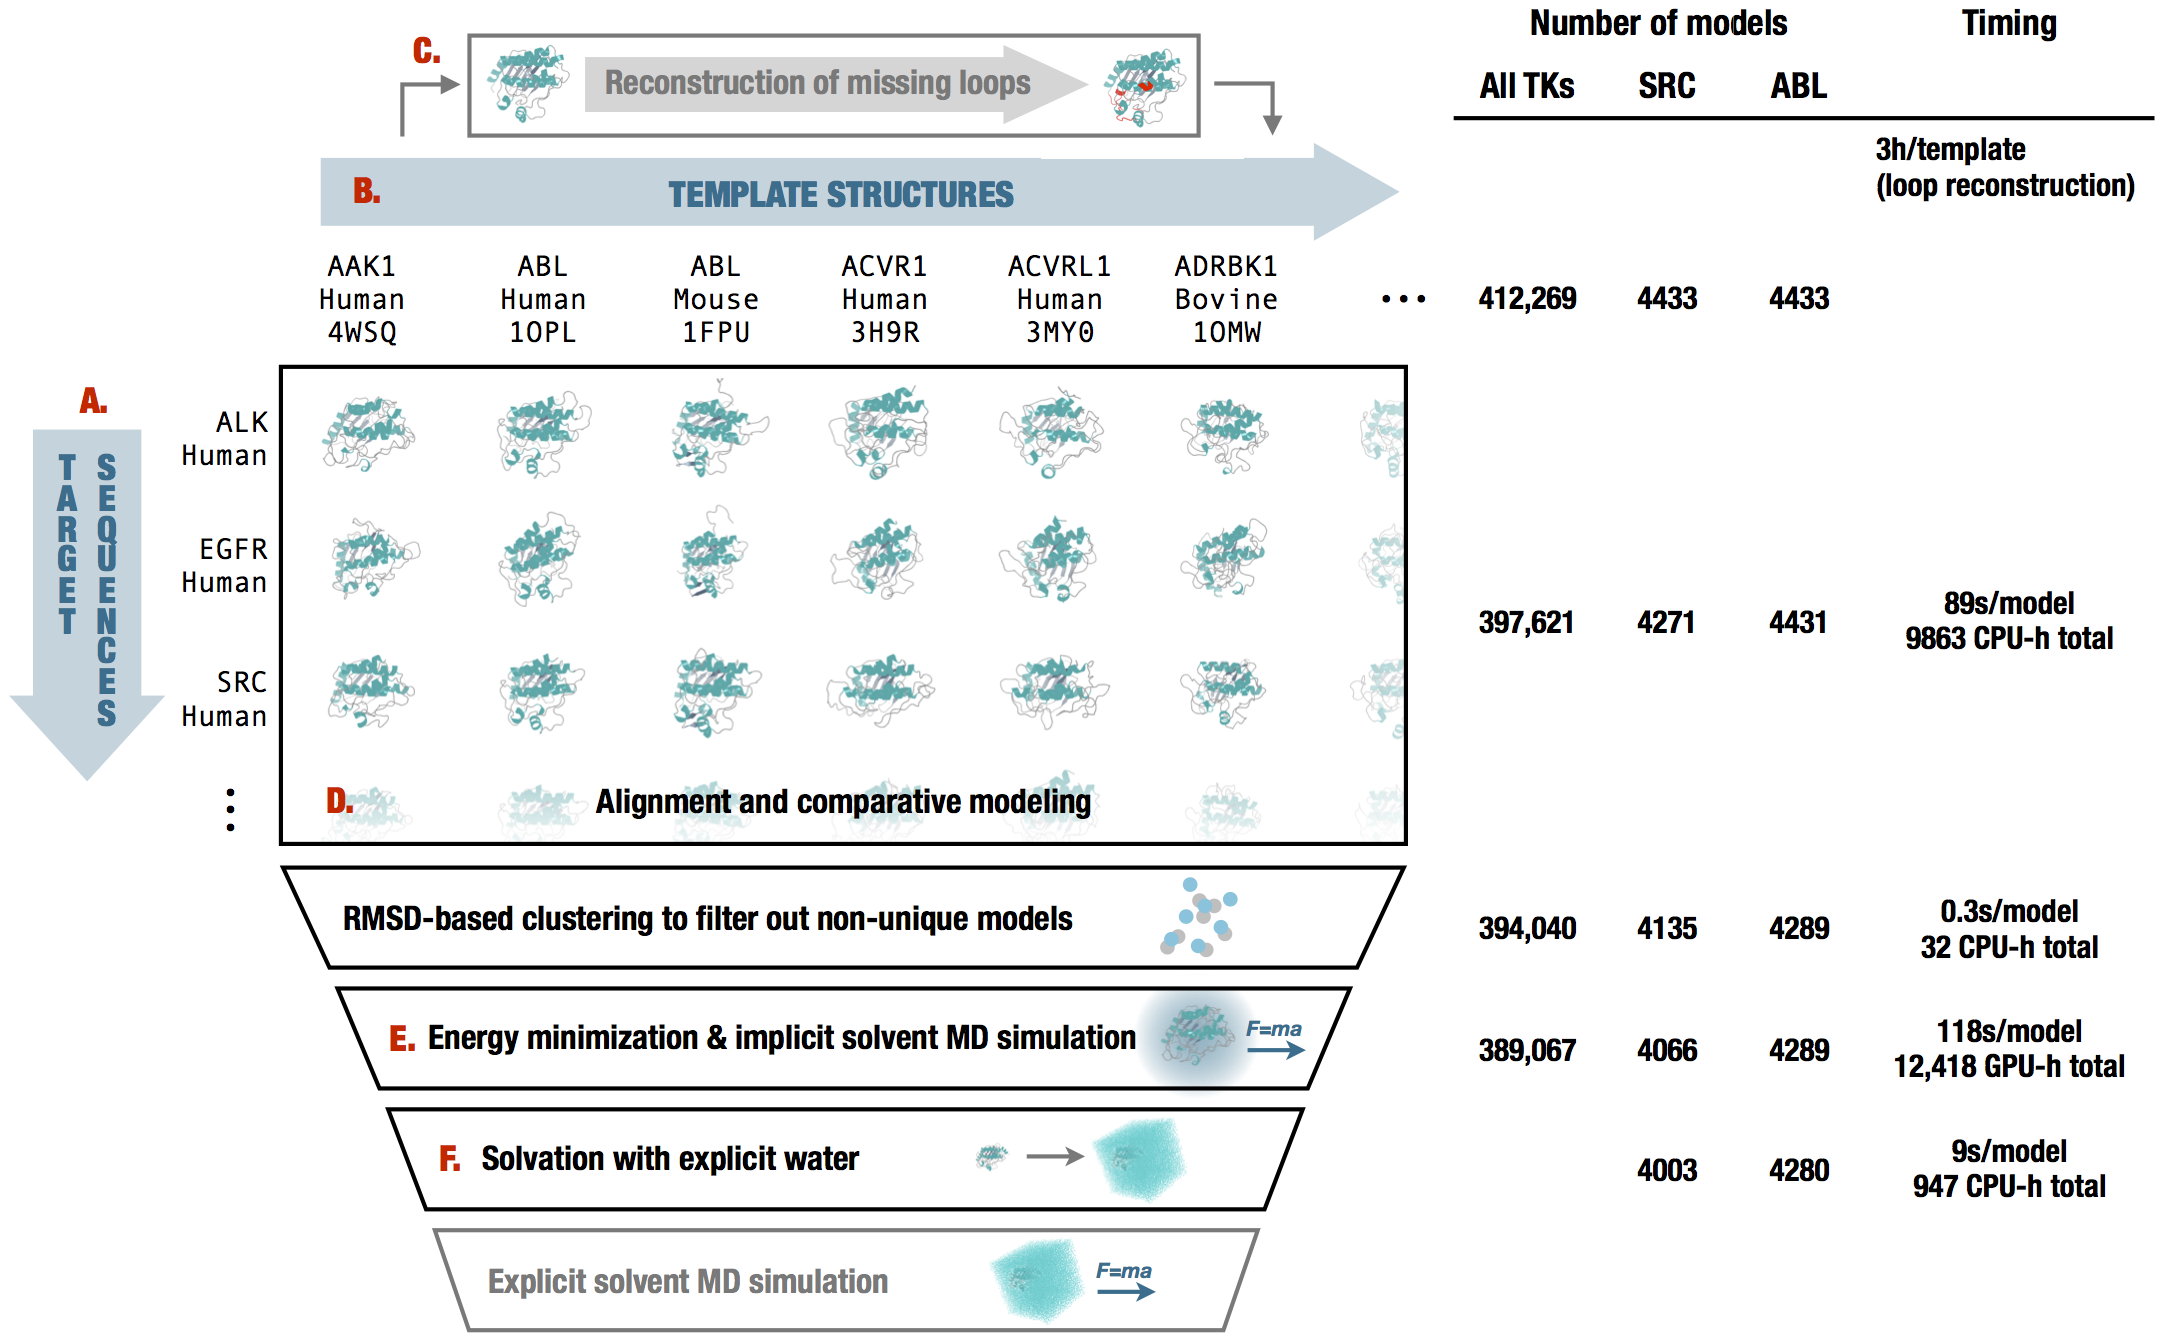
\includegraphics[width=1.0\textwidth]{pipeline2}
  \caption{{\bf Diagrammatic representation of the various stages of the Ensembler pipeline.}
  The number of viable models surviving each stage of the pipeline for are shown, either for all tyrosine kinases (\emph{All TKs}) or representative individual kinases (\emph{SRC} and \emph{ABL}).
  In addition, the typical timing on a cluster (containing Intel Xeon E5-2665 2.4GHz hyperthreaded processors and NVIDIA GTX-680 or GTX-Titan GPUs) is reported to convey resources required per model and for modeling the entire set of tyrosine kinases.
  Note that \emph{CPU-h} denotes the number of hours consumed by the equivalent of a single hyperthread---parallel execution can reduce wall clock time nearly linearly.
  }
  \label{figpipeline}
\end{figure*}

\subsubsection{Target selection}

The first stage entails the selection of a set of target protein sequences.

These targets can be defined manually, simply by providing a FASTA-formatted text file containing the desired target sequences with arbitrary identifiers.
The {\tt ensembler} command-line tool also allows targets to be selected from UniProt---a freely accessible resource for protein sequence and functional data (\href{http://www.uniprot.org/}{uniprot.org}), using the subcommand {\tt gather\_targets}.
% {\color{red}[JDC: Does it make sense to omit discussion of TargetExplorer since it's not clear how useful this will be to users?]}
% {\color{blue}[DLP: Yes, I think TargetExplorer is primarily an internal tool for the moment, so let's omit discussion of that.]}
The user specifies a query string with the {\tt -{}-query} flag, which conforms to the same syntax as the search function available on the UniProt website.
% {\color{red}[JDC: What command-line flag or API call is used to select targets from UniProt?]}
% {\color{red}[DLP: the command-line flag is now described]}
For example, {\tt -{}-query `mnemonic:SRC\_HUMAN'} would select the full-length human Src sequence, while {\tt -{}-query `domain:"Protein kinase" AND taxonomy:9606 AND reviewed:yes'} would select all human protein kinases which have been reviewed by a human curator.
In this way, the user may select a single protein, many proteins, or an entire superfamily.
The program outputs a FASTA file, setting the UniProt mnemonic (e.g. {\tt SRC\_HUMAN}) as the identifier for each target protein.
% {\color{red}[JDC: Can you give a clearer picture of how this is done?  Does the user just specify different flags for these categories, or would they have to construct different Uniprot searches?]}
% {\color{blue}[DLP: This is explained more clearly now.]}

In many cases, it will be desirable to build models of an isolated protein domain, rather than the full-length protein.
The {\tt gather\_targets} subcommand allows protein domains to be selected from UniProt data by passing a regular expression string to the {\tt -{}-domains} flag. 
For example, the above {\tt -{}-query} flag for selecting all human protein kinases returns UniProt entries with domain annotations including "Protein kinase", "Protein kinase 1", "Protein kinase 2", "Protein kinase; truncated", "Protein kinase; inactive", "SH2", "SH3", etc.
To select only domains of the first three types, the following regular expression could be used: {\tt`\^{}Protein kinase(?!; truncated)(?!; inactive)'}.
In this case, target identifiers are set with the form {\tt [UniProt mnemonic]\_D[domain index]}, where the latter part represents a 0-based index for the domain---necessary because a single target protein may contain multiple domains of interest.
Example identifiers: {\tt JAK1\_HUMAN\_D0}, {\tt JAK1\_HUMAN\_D1}.

\subsubsection{Template selection}

The second stage entails the selection of templates and storage of associated structures, sequences and identifiers.

This data can be provided manually, by storing the sequences and identifiers in a FASTA file, and the structures as PDB-format coordinate files with filenames matching the identifiers in the sequence file.
The structure residues must also match those in the sequence file.

The {\tt ensembler gather\_templates} subcommand also provides methods for selecting template structures from either UniProt or the Protein Data Bank (PDB; \href{http://www.rcsb.org/pdb}), specified by the {\tt -{}-gather\_from} flag.

% {\color{red}[JDC: Do you use the RCSB or some other PDB site?]} - DLP: I use the RCSB, but all PDB sites are updated simultaneously so I think it shouldn't matter. However, I've updated the link so that it points to the RCSB PDB.
% {\color{red}[JDC: Again, not sure if it is helpful to leave this in unless it will be immediately useful to the reader]} - DLP: references to TargetExplorer removed

Selection of templates from the PDB simply requires passing a list of PDB IDs as a comma-separated string, e.g. {\tt -{}-query 2H8H,1Y57}.
% {\color{red}[JDC: Who specifies the list of PDB IDs?  How are they specified?  Can this be built automatically, or does the user need to specify these?]} DLP: these are specified by the user as a comma-separated list, as is now described above.
Specific PDB chain IDs can optionally also be selected via the {\tt -{}-chainids} flag.
The program retrieves structures from the PDB server, as well as associated data from the SIFTS service (\href{http://www.ebi.ac.uk/pdbe/docs/sifts/}{www.ebi.ac.uk/pdbe/docs/sifts}) (CITE: Velankar Nucleic Acids Res 2013), which provides residue-level mappings between PDB and UniProt entries.
The SIFTS data is used to extract template sequences, retaining only residues which are resolved and match the equivalent residue in the UniProt sequence---non-wildtype residues are thus removed from the template structures.
Furthermore, PDB chains with less than a given percentage of resolved residues (default: 70\%) are filtered out.
Sequences are stored in a FASTA file, with identifiers of the form {\tt [UniProt mnemonic]\_D[UniProt domain index]\_[PDB ID]\_[PDB chain ID]}, e.g. {\tt SRC\_HUMAN\_D0\_2H8H\_A}.
Template structures with residues matching the sequence data are then extracted and stored as PDB-format coordinate files.

Selection of templates from UniProt proceeds in a similar fashion as for target selection; the {\tt -{}-query} flag is used to select full-length proteins from UniProt, while the optional {\tt -{}-domains} flag allows selection of individual domains with a regular expression string.
The returned UniProt data for each protein includes a list of associated PDB chains and their residue spans, and this information is used to select template structures, using the same method as for template selection from the PDB.
If the {\tt -{}-domains} flag is used, then templates are truncated at the start and end of the domain sequence.

Unresolved template loops can optionally be remodeled with a kinematic closure algorithm {\color{red}[CITE]}, which is provided via the loopmodel tool of the Rosetta software suite (CITE: Rosetta and/or loopmodel).
Because fewer loops need to be built during the subsequent model-building stage, prebuilding template loops tends to provide higher-quality models following the subsequent modeling process.

\subsubsection{Modeling}

This stage entails the generation of models via comparative modeling of each target sequence onto each template structure. Non-unique models are filtered out using a RMSD-based clustering scheme.

Modeling is performed with the Modeller automodel function {\color{red}[CITE: Modeller]}, which implements comparative structure modeling by satisfaction of spatial restraints {\color{red}[CITE: Sali Blundell J Mol Biol 1993; Fiser Sali Prot Sci 9 2000]}.
While Modeller can generate alignments automatically, we utilize the BioPython {\tt pairwise2} module (CITE: BioPython)---which uses a dynamic programming algorithm---with the PAM 250 scoring matrix of Gonnet \textit{et al.}~{\color{red}[CITE: Gaston Gonnet Science 1992]}, which we have empirically found to produce better quality alignments for purposes of high-throughput model building.

All chains of template structures that contain the template sequence are utilized in the modeling phase, which can sometimes cause models to be nearly identical.
Since the goal is to provide good coverage of conformation space, {\bf Ensembler} filters out nearly identical models using structural similarity-based clustering.
The mdtraj {\color{red}[CITE: mdtraj]} Python library is used to calculate RMSD (for C$\alpha$ atoms only) with a fast quaternion characteristic polynomial (QCP)~{\color{red}[Cite Theobald QCP papers]} implementation, and the leader algorithm is then used to populate clusters.
A minimum distance cutoff (which defaults to 0.6 \AA) is used to retain only a single model per cluster.
% {\color{red}[JDC: Which atoms are used in the RMSD comparison?  All atoms, heavy atoms, or CA only?]} - DLP: CA only. This is now specified in the text.

\subsubsection{Refinement}

This stage entails the use of molecular dynamics simulations to refine the models built in the previous step.
This helps to improve model quality and also prepares models for subsequent production simulation, including solvation with explicit water molecules, if desired.

Models are first subjected to energy minimization (using the L-BFGS algorithm {\color{red}[CITE]}), followed by a short molecular dynamics (MD) simulation with an implicit solvent representation.
This is implemented using the OpenMM molecular simulation toolkit (link and CITE: OpenMM), chosen for its flexible Python API, and high performance GPU-acclerated simulation code.
By default, the Amber99SB-ILDN force field is used {\color{red}[CITE: amber99sbildn refs]} with a modified generalized Born solvent model (GBSA-OBC) (CITE: GBSA-OBC).
The {\bf Ensembler} API allows the use of any of the other force fields implemented in OpenMM.
The simulation is run for a default of 100 ps to filter out poor quality models (where atomic overlaps that cannot be resolved by energy minimization would cause the simulation to explode) and help relax models for subsequent production simulation.
{\color{red}[JDC: What criteria were applied to filter out poor models?  Do we only look for thrown exceptions or NaNs?  Or do we use an energy filtering criteria too?]}
{\color{blue}[DLP: We currently just filter out models which throw exceptions or NaNs.]}

While protein-only models may be sufficient for structural analysis or implicit solvent simulations, {\bf Ensembler} also provides a stage for solvating models with explicit water and performing a round of explicit-solvent MD refinement/equilibration under isothermal-isobaric (NPT) conditions.
The solvation step solvates each model for a given target with the same number of waters to facilitate the integration of data from multiple simulations, such as the construction of MSMs.
The target number of waters is selected by first solvating each model with a specified padding distance (default: 10 \AA), then taking a percentile value from the distribution (default: 68th percentile).
{\color{red}[JDC: Would be useful to explain why we are doing this.]}
{\color{blue}[DLP: Addressed.]}
This helps to prevent models with particularly long, extended loops---such as those arising from template structures with unresolved termini---from imposing very large box sizes on the entire set of models.
Models are resolvated with the target number of waters by first solvating with zero padding, then incrementally increasing the box size and resolvating until the target is exceeded, then finally deleting sufficient waters to match the target value.
The explicit solvent MD simulation is also implemented using OpenMM, using the Amber99SB-ILDN force field and TIP3P water {\color{red}[JDC: CITE]} by default.
Other force fields or water models such as TIP4P-Ew {\color{red}[CITE]}) can be specified via the {\bf Ensembler} API.
{\color{red}[JDC: We should allow other water models in OpenMM too, such as TIP4P-Ew?]}
{\color{blue}[DLP: I forgot to mention this in the text previously - any of the OpenMM force fields can be chosen via the API. I've updated the text accordingly. Is this functionality sufficient? I guess it's ok to leave ff choice as an "advanced" feature which requires use of the API? Otherwise I could add a --water\_model flag to the CLI, for example.]}

{\color{red}[JDC: In the Discussion, let's be sure to talk about the limitations and what could be improved or added in the future.  For example, we don't yet handle counterions (e.g. structural Zn$^{2+}$), prosthetic groups (e.g.~heme), or cofactors (e.g.~ATP) yet.  We don't handle post-translational modifications either (such as phosphorylation, methylation, glycosylation, etc.).  It's a good idea to suggest that this is an important first step toward enabling superfamily- and genomics-scale modeling, but there's a lot of work yet to be done.]}

\subsubsection{Packaging}

{\bf Ensembler} provides a packaging module which can be used to compress models in preparation for data transfer, or to prepare models with the appropriate directory and file structure for subsequent production simulations on the distributed computing platform Folding@home (CITE: F@H).

\subsubsection{Provenance}

To aid the user in tracking the provenance of each model, each pipeline function also outputs a metadata file, which helps to link data to the software version used to generate it (both {\bf Ensembler} and its dependencies), and also provides timing and performance information, and other data such as hostname.

\subsubsection{Rapidly modeling a single template}

% quickmodel function performs the entire pipeline in one go, for a single target and a small number of templates.
For users interested in simply using {\bf Ensembler} to rapidly generate a set of models for a single template sequence, {\bf Ensembler} provides a command-line tool {\tt quickmodel}, which performs the entire pipeline for a single target with a small number of templates.
For larger numbers of models (such as entire protein families), modeling time is greatly reduced by using the main modeling pipeline, which is parallelized via MPI, distributing computation across each model (or across each template, in the case of the loop reconstruction code), and scaling (in a ``pleasantly parallel'' manner) up to the number of models generated.


% ? The API is highly flexible, allowing control over many important parameters. Appropriate choices have been set as default values.



% TODO where do these go?
% Distribution: conda package or github source
% Software is open source and designed to be extensible as far as possible. For example, it would be very simple to implement further options for providing target and template structures, or for packaging models.


\label{section:design}

%%%%%%%%%%%%%%%%%%%%%%%%%%%%%%%%%%%%%%%%%%%%%%%%%%%%%%%%%%%%%%%%%%%%%%%%%%%%%%%%%%%%%%%%%%%%%%%%%%%%%
% RESULTS
%%%%%%%%%%%%%%%%%%%%%%%%%%%%%%%%%%%%%%%%%%%%%%%%%%%%%%%%%%%%%%%%%%%%%%%%%%%%%%%%%%%%%%%%%%%%%%%%%%%%%
\section{Results}
\label{section:results}

% \begin{table}
% \begin{tabular}{l|c|c|c}
%
%     & SRC & ABL & All 90 TKs \\
%     \hline
%     Templates & \num{4433} & \num{4433} & \num{398970} \\
%     Models & \num{4248} & \num{4250} & \num{382568} \\
%     Unique models & \num{4093} & \num{4247} & \num{378839} \\
%     Refined models & \num{4023} & \num{4241} & \num{373513} \\
%
% \end{tabular}
% \label{tab:model_counts}
% \caption{Model counts for the kinase domains of human SRC and ABL, and for all of the 90 human TK targets, at various stages of the Ensembler pipeline.}
% \end{table}
%
% \begin{table}
% \begin{tabular}{l|c}
%
%     & Timing ($h$:$m$:$s$) \\
%     \hline
%     Template reconstruction & 03:00:00 \\
%     Modeling & 00:01:19 \\
%     Refinement (100 ps implicit solvent MD) & 00:01:58 \\
%
% \end{tabular}
% \label{tab:timings}
% \caption{Average timings per template/model for the compute-intensive stages of the Ensembler pipeline.}
% \end{table}

%%%%%%%%%%%%%%%%%%%%%%%%%%%%%%%%%%%%%%%%%%%%%%%%%%%%%%%%%%%%%%%%%%%%%%%%%%%%%%%%%%%%%%%%%%%%%%%%%%%%%
% DISCUSSION
%%%%%%%%%%%%%%%%%%%%%%%%%%%%%%%%%%%%%%%%%%%%%%%%%%%%%%%%%%%%%%%%%%%%%%%%%%%%%%%%%%%%%%%%%%%%%%%%%%%%%
\section{Availability and Future Directions}
\label{section:availability}

%%%%%%%%%%%%%%%%%%%%%%%%%%%%%%%%%%%%%%%%%%%%%%%%%%%%%%%%%%%%%%%%%%%%%%%%%%%%%%%%%%%%%%%%%%%%%%%%%%%%%
% ACKNOWLEDGMENTS
%%%%%%%%%%%%%%%%%%%%%%%%%%%%%%%%%%%%%%%%%%%%%%%%%%%%%%%%%%%%%%%%%%%%%%%%%%%%%%%%%%%%%%%%%%%%%%%%%%%%%
\section{Acknowledgments}
\label{section:acknowledgments}

The authors are grateful to Kyle A.~Beauchamp (MSKCC), Robert McGibbon (Stanford), Arien S. Rustenburg (MSKCC) for many excellent software engineering suggestions.
The authors thank Sonya M.~Hanson (MSKCC), Nicholas M.~Levinson (?), Markus A.~Seeliger (Stony Brook), Diwakar Shukla (Stanford), and Avner Schlessinger (Mount Sinai) for helpful scientific feedback on modeling kinases.
The authors are grateful to Benjamin Webb and Andrej Sali (UCSF) for help with the MODELLER package, Peter Eastman and Vijay Pande (Stanford) for assistance with OpenMM, and Marilyn Gunner (CCNY) for assistance with MCCE2.
DLP and this work was supported in part by the generous support of a Louis V.~Gerstner Young Investigator Award.

%%%%%%%%%%%%%%%%%%%%%%%%%%%%%%%%%%%%%%%%%%%%%%%%%%%%%%%%%%%%%%%%%%%%%%%%%%%%%%%%%%%%%%%%%%%%%%%%%%%%%%
% BIBLIOGRAPHY
%%%%%%%%%%%%%%%%%%%%%%%%%%%%%%%%%%%%%%%%%%%%%%%%%%%%%%%%%%%%%%%%%%%%%%%%%%%%%%%%%%%%%%%%%%%%%%%%%%%%%%

%\bibliographystyle{prsty} 
\bibliography{ms.bib}

\end{document}
